\documentclass[submit]{harvardml}

\course{CS181-S23}
\assignment{Assignment \#1}
\duedate{11:59pm ET, February 9, 2023} 

\usepackage[OT1]{fontenc}
\usepackage[colorlinks,citecolor=blue,urlcolor=blue]{hyperref}
\usepackage[pdftex]{graphicx}
\usepackage{graphicx}
\usepackage{caption}
\usepackage{fullpage}
\usepackage{enumitem}
\usepackage{soul}
\usepackage{amsmath}
\usepackage{amssymb}
\usepackage{color}
\usepackage{todonotes}
\usepackage{listings}
\usepackage{common}
\usepackage{framed}
\usepackage{float}

\usepackage[mmddyyyy,hhmmss]{datetime}

\definecolor{verbgray}{gray}{0.9}

\lstnewenvironment{csv}{
  \lstset{backgroundcolor=\color{verbgray},
  frame=single,
  framerule=0pt,
  basicstyle=\ttfamily,
  columns=fullflexible}}{}

 \DeclareMathOperator*{\limover}{\overline{lim}}

\begin{document}
\begin{center}
{\Large Homework 1: Regression}\\
\end{center}

\subsection*{Introduction}
This homework is on different three different forms of regression: kernelized regression, nearest neighbors regression, 
and linear regression.  We will discuss implementation and examine their tradeoffs by implementing them on the same dataset, 
which consists of temperature over the past 800,000 years taken from ice core samples.

The folder \verb|data| contains the data you will use for this problem. There are two files:
\begin{itemize}
    \item \verb|earth_temperature_sampled_train.csv| 
    \item \verb|earth_temperature_sampled_test.csv|
\end{itemize} 

Each has two columns.  The first column is the age of the ice core sample. For our purposes we can 
think of this column as the calendar year BC. The second column is the approximate difference in 
yearly temperature (K) from the mean  over a 5000 year time window starting at the given age. 
The temperatures were retrieved from ice cores in Antarctica (Jouzel 
et al. 2007)\footnote{Retrieved from \url{https://www.ncei.noaa.gov/pub/data/paleo/icecore/antarctica/epica_domec/edc3deuttemp2007.txt}


Jouzel, J., Masson-Delmotte, V., Cattani, O., Dreyfus, G., Falourd, 
S., Hoffmann, G., … Wolff, E. W. (2007). Orbital and Millennial 
Antarctic Climate Variability over the Past 800,000 Years. 
\emph{Science, 317}(5839), 793–796. doi:10.1126/science.1141038}.
 
 The following is a snippet of the data file:
 
\begin{csv}
# Age, Temperature
3.999460000000000000e+05,5.090439218398755017e+00
4.099800000000000000e+05,6.150439218398755514e+00
\end{csv}

\textbf{Due to the large magnitude of the years, we will work in terms of thousands of years BCE in Problems 1-3.} This is taken care of for you in the provided notebook.

\begin{center}
\includegraphics[width=.8\textwidth]{images/temperature}
\end{center}
\noindent 


If you find that you are having trouble with the first couple
problems, we recommend going over the fundamentals of linear algebra
and matrix calculus (see links on website).  The relevant parts of the
\href{https://github.com/harvard-ml-courses/cs181-textbook/blob/master/Textbook.pdf}{cs181-textbook notes are Sections 2.1 - 2.7}.  We strongly recommend
reading the textbook before beginning the homework.

We also encourage you to first read the \href{http://users.isr.ist.utl.pt/~wurmd/Livros/school/Bishop\%20-\%20Pattern\%20Recognition\%20And\%20Machine\%20Learning\%20-\%20Springer\%20\%202006.pdf}{Bishop textbook}, particularly:
Section 2.3 (Properties of Gaussian Distributions), Section 3.1
(Linear Basis Regression), and Section 3.3 (Bayesian Linear
Regression). (Note that our notation is slightly different but the
underlying mathematics remains the same!).

\textbf{Please type your solutions after the corresponding problems using this
\LaTeX\ template, and start each problem on a new page.} You may find
the following introductory resources on \LaTeX\ useful: 
\href{http://www.mjdenny.com/workshops/LaTeX_Intro.pdf}{\LaTeX\ Basics} 
and \href{https://www.overleaf.com/learn/latex/Free_online_introduction_to_LaTeX_(part_1)}{\LaTeX\ tutorial with exercises in Overleaf}

Homeworks will be submitted through Gradescope. You will be added to
the course Gradescope once you join the course Canvas page. If you
haven't received an invitation, contact the course staff through Ed.

\textbf{Please submit the writeup PDF to the Gradescope assignment
  `HW1'.} Remember to assign pages for each question.

\textbf{Please submit your \LaTeX file and code files to the
  Gradescope assignment `HW1 - Supplemental'.} Your files should be
named in the same way as we provide them in the repository,
e.g. \texttt{hw1.pdf}, etc.


%%%%%%%%%%%%%%%%%%%%%%%%%%%%%%%%%%%%%%%%%%%%%
% Problem 1
%%%%%%%%%%%%%%%%%%%%%%%%%%%%%%%%%%%%%%%%%%%%%
\begin{problem}[Optimizing a Kernel]
Kernel-based regression techniques are similar to nearest-neighbor
regressors: rather than fit a parametric model, they predict values
for new data points by interpolating values from existing points in
the training set.  In this problem, we will consider a kernel-based
regressor of the form:
\begin{equation*}
  f_\tau(x^*) = \cfrac{\sum_{n} K_\tau(x_n,x^*) y_n}{\sum_n K_\tau(x_n, x^*)} 
\end{equation*}
where $\{(x_n,y_n)\}_{n = 1} ^N$ are the training data points, and $K_\tau(x,x')$ is a
kernel function that defines the similarity between two inputs $x$ and
$x'$. A popular choice of kernel is a function that decays as the
distance between the two points increases, such as
\begin{equation*}
  K_\tau(x,x') = \exp\left\{-\frac{(x-x')^2}{\tau}\right\}
\end{equation*}
where $\tau$ represents the square of the lengthscale (a scalar value that 
dictates how quickly the kernel decays).  In this
problem, we will consider optimizing what that (squared) lengthscale
should be.

\noindent\emph{Make sure to include all required plots in your PDF.}

\begin{enumerate}
  
\item Let's first take a look at the behavior of the fitted model for different values of $\tau$. Plot your model for years in the range $800,000$ BC to $400,000$ BC at $1000$ year intervals for the following three values of $\tau$: $1, 50, 2500$. Since we're working in terms of thousands of years, this means you should plot $(x, f_\tau(x))$ for $x = 400, 401, \dots, 800$. The plotting has been set up for you in the notebook already.


Include your plot in your solution PDF.

\textbf{In no more than 5 sentences}, describe what happens in each of the three cases. How well do the models interpolate? If you were to choose one of these models to use for predicting the temperature at some year in this range, which would you use? 

\item Say we instead wanted to empirically evaluate which value of $\tau$ to choose. One option is to evaluate the mean squared error (MSE) for $f_{\tau}$ on the training set and simply choose the value of $\tau$ that gives the lowest loss. Why is this a bad idea?
    
Hint: consider what value of $\tau$ would be optimal, for $\tau$ ranging in $(0, \infty)$. We can consider $f_\tau(x^*)$ as a weighted average of the training responses, where the weights are proportional to the distance to $x^*$, and the distance is computed via the kernel. What happens to $K_\tau(x, x')$ as $\tau$ becomes very small, when $x = x'$? What about when $x \neq x'$?

\item We will evaluate the models by computing their MSE on the test set. 

Let $\{(x'_m, y'_m)\}_{m = 1} ^M$ denote the test set. Write down the form of the MSE of $f_\tau$ over the test set as a function of the training set and test set. Your answer may include $\{(x'_m, y'_m)\}_{m = 1} ^M$, $\{(x_n, y_n)\}_{n = 1} ^N$, and $K_\tau$, but not $f_\tau$.

\item We now compute the MSE on the provided test set. Write Python code to compute the MSE with respect to the same lengthscales as in Part 1. Which model yields the lowest test set MSE? Is this consistent with what you observed in Part 1?

\item 
Say you would like to send your friend your kernelized regressor, so that they can reproduce the same exact predictions as you. You of course will tell them the value of $\tau$ you selected, but what other information would they need, assuming they don't currently have any of your data or code? If our training set has size $N$, how does this amount of information grow as a function of $N$—that is, what is the space complexity of storing our model?

What is the time complexity of your implementation, when computing your model on a new datapoint? 
\end{enumerate}

\end{problem}

\newpage

\textbf{Problem 1 Solution:}\\
\begin{enumerate}
    \item 
    Behavior of the fitted model for different values of $\tau$:\\
    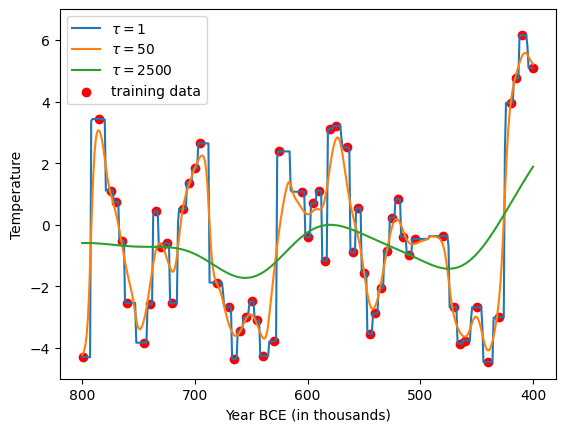
\includegraphics[scale=0.8
    ]{hw1/KernelGraph.png}\\
    From this graph we can clearly see that when $\tau=2500$ our model is underfitting our data and not accounting for any of the noise. It has a high bias with a low variance. On the other hand, when $\tau=1$ our model is overfitting the data because it is accounting for every one of our noisy points. It has a low bias and high variance. $\tau=50$ seems like the best option out of the three because it manages the bias/variance tradeoff the best: it is following our training data but is not too extreme where it hits every point and overfits.\\ 
    \item\\
    We do not want to evaluate the mean squared error for $f_{\tau}$  on the training set and give the value of $\tau$ that minimizes the loss because then we would be overfitting our data. In this example we would be only looking at the training set so we would fit the training set really well but that doesn't necessarily mean that it will fit our test data very well. If we were to use this strategy a value of $\tau=0$ would be the optimal solution but just like $\tau=1$ this would overfit our data (it would prioritize variance much more than bias). If $\tau$ becomes very small when $x=x'$ then $K_{\tau}$ would be equal to $e^0=1$ and when $x\neq x'$, our exponent of $e$ would get very big so $K_{\tau}$ would get closer and closer to 0.\\
    \item\\
    First we can start with the standard MSE equation:
    \begin{equation*}
       \texttt{MSE} = \frac{1}{N} \sum_{i=1}^N\left(y_i - \hat{y_i}\right)^2
    \end{equation*}\\
    We know that we are calculating our MSE on the $M$ test values. Our true values will be the true values in the test test ($y'_m$) and our predicted values will be based on inputting our $x'_m$ into our kernel equation (summing through our training data points). This means our specific MSE equation is:\\
    \begin{equation*}
       \texttt{MSE} = \frac{1}{M} \sum_{m=1}^M\left(y'_m - \cfrac{\sum_{n} K_\tau(x_n,x^{'}_m) y_n}{\sum_n K_\tau(x_n, x^{'}_m)} \right)^2
    \end{equation*}\\
    \item\\
    I next computed the MSE on the training data set for different values of $\tau$:\\
    tau = 1: loss = 1.9472621565209178\\
    tau = 50: loss = 1.8582899169613452\\
    tau = 2500: loss = 8.333886806980793\\
    From this data we can clearly see that $\tau=50$ yields the lowest test set MSE. This is consistent with what I observed in Part 1, because I thought that $\tau=1$ was overfitting (so would not have a low MSE on the test data) and $\tau=2500$ was underfitting so it also would not have a good MSE on the test data.\\
    \item\\
    Aside from just the value of $\tau$ that I selected, I would send my friend what kernel function I used and the training data points I used to train my model. The space complexity of storing our model would be $O(N)$ because we would need to store the $N$ data points. When computing my model on a new datapoint, the time complexity is $O(N)$. Whenever we add a new datapoint we know that we need to implement our kernel function on my new data point against each of the other training points. This function is $O(1)$ and we are doing it $O(N)$ times so overall the time complexity is $O(N)$.

\end{enumerate}

\newpage


%%%%%%%%%%%%%%%%%%%%%%%%%%%%%%%%%%%%%%%%%%%%%
% Problem 2
%%%%%%%%%%%%%%%%%%%%%%%%%%%%%%%%%%%%%%%%%%%%%

\begin{problem}[Kernels and kNN]

Now, let us compare the kernel-based approach to an approach based on
nearest-neighbors.  Recall that kNN uses a predictor of the form
  \begin{equation*}
    f(x^*) = \frac{1}{k} \sum_n y_n \mathbb{I}(x_n \texttt{ is one of k-closest to } x^*)
  \end{equation*}

\noindent where $\mathbb{I}$ is an indicator variable. For this problem, you will use the \textbf{same dataset as in Problem 1}.


%\textbf{For this problem, you may also use the second half of the notebook at {\color{red} update name} \texttt{T1\_P1-2.ipynb}.} 

\textbf{Note that our set of test cases is not comprehensive: just because you pass does not mean your solution is correct! We strongly encourage you to write your own test cases and read more about ours in the comments of the Python script.}

\vspace{0.5cm}
\noindent\emph{Make sure to include all required plots in your PDF.}


\begin{enumerate}

\item Implement kNN for $k=\{1, 3, N-1\}$ where $N$ is the size of the dataset, then plot the results for each $k$. To find the distance between points, use the kernel function from Problem 1 with lengthscale $\tau=2500$. 

You will plot $x^*$ on the year-axis and the prediction $f(x^*)$ on the temperature-axis.  For the test inputs $x^*$, you should use an even grid spacing of $1$ between $x^* = 800$ and $x^* = 400$.  (Like in Problem 1, if a test point lies on top of a training input, use the formula without excluding that training input.) Again, this has been set up for you already.

Please \textbf{write your own
    implementation of kNN} for full credit.  Do not use external
  libraries to find nearest neighbors.
  
\item Describe what you see: what is the behavior of the functions in
  these three plots?  How does it compare to the behavior of the
  functions in the three plots from Problem 1? In particular, which of the plots from Problem 1 look most similar to each in Problem 2? Are there situations
  in which kNN and kernel-based regression interpolate similarly?

\item Choose the kNN model you most prefer among the three. Which model did you choose and why? What is its mean squared error on the test set?

\item As before, say you wanted to send your friend your kNN, so that they can reproduce the same exact predictions as you. You will again tell them the value of the $k$ you selected, but what other information would they need, assuming they do not currently have any of your data or code, and how does this information grow as a function of the size of the training set, $N$? Again worded more formally, what is the space complexity of storing your model?

What is the time complexity of your implementation, when computing your model on a new datapoint? Give a brief overview of your implementation when you justify your answers. 
\end{enumerate}

\end{problem}
\newpage
\textbf{Problem 2 Solution:}\\
\begin{enumerate}
    \item  Behavior of the fitted model for different values of $k$:\\
    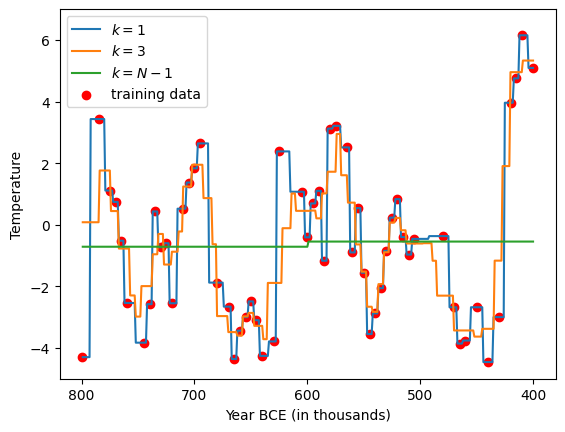
\includegraphics[scale=0.8
    ]{hw1/knnGraph.png}\\
    (I added an additional test case to check my implementation and this is included in my code file).\\
    \item\\
    From this graph we can that when $k=1$ our graph seems to fit every point in the data. This behavior is very similar to the behavior of the graph of $\tau=1$ in part 1 because they both fit every point in the training data (they are both overfitting the data). The graph for $k=N-1$ is almost a flat line and it seems to match the behavior of $\tau=2500$ from part 1. Both of these models underfit our data. Lastly, $k=3$ looks like it is interpolating best as it is accounting for the variation from the noise is our data without fitting it exactly. It is the best at balancing the bias/variance tradeoff(not overfitting or underfitting too much). It's behavior is most similar to the model when $\tau=50$ in part 1. Overall, the behavior of the two models (part 1 and part 2) do behave similarly. Furthermore, we know that in part 1, as $\tau \rightarrow \infty$ the green line would continue to become flatter and look even more similar to the graph of $k=N-1$. \\
    \item
    When just looking at the graph my initial thought was that the $k=3$ model would be optimal because it seems to do the best with balancing the bias/variance tradeoff (not overfitting or underfitting the data). It is able to account for noise (which $k=N-1$ does not) but it does not fit every single training data point like the model of $k=1$.\\
    \\
    However, in my code I was able to actually calculate the mean squared error of each model on the test set. These are my results:\\
    k = 1: loss = 1.7406000000000004\\
    k = 3: loss = 3.8907662222222212\\
    k = N -1: loss = 9.528571442602042 \\
    \\
    Interestingly, these results show that $k=1$ has the lowest value of loss (different from my original prediction). This model chooses a low bias in exchange for a higher variance. Perhaps in this case because of the data we are using, $k=1$ is the optimal choice. From the image of the true temperature trends provided to us we can see that the test data does seem to be very similar to the training data, so when we use $k=1$ we are not overfitting our model, but instead fitting it optimally for this test data. Additionally, because our data is covering millions of years and using averages, $k=3$ could be in fact underfitting. As a result, I would ultimately say that the model with $k=1$ is optimal.\\
    \item
    Aside from telling my friend the value of $k$ that I selected, I would also send them the training data points I used. Similarly as in problem 1, the space complexity of storing our model would be $O(N)$ because we need to store all of our training data points. Our time complexity of computing this model on a new data point would be longer than in question 1 because each step in our algorithm requires a little bit more work. For each data point, we need to calculate its distance from all of the other training data points. We then need to sort these distances so we know which $k$ are closest. Lastly, we sum our value of $y$ for each the $k$ points that are closest.The longest step of this process is actually sorting our data which I am doing in $O(N\cdot \log N)$ time (we know this takes the longest because calculating every distance would just be using our Kernel function $N$ times so this would take $O(N)$ time). This means the overall process would take $O(N\cdot \log N)$ time. \\
    (As an aside, if I were able to implement a faster sorting method such as the median of medians approach then I could possibly make this sorting process faster so that the overall process would only take $O(N)$ time).\\
    
\end{enumerate}

%%%%%%%%%%%%%%%%%%%%%%%%%%%%%%%%%%%%%%%%%%%%%
% Problem 3
%%%%%%%%%%%%%%%%%%%%%%%%%%%%%%%%%%%%%%%%%%%%%

\newpage
\begin{problem}[Modeling Climate Change 800,000 Years Ago]

 The objective of this problem is to learn about different forms of
 linear regression with basis functions.

\vspace{1em}
\noindent\emph{Make sure to include all required plots in your PDF.}

\begin{enumerate}
\item 
Recall that in \emph{Ordinary Least Squares} (OLS) regression,
we have data $\{(\mathbf{x}_i, y_i)\}_{i=1}^N = \{\mathbf{X}, \mathbf{y}\}$ 
where $\mathbf{X} \in \mathbb{R}^{N\times D}$. The goal is to find 
the weights $\mathbf{w} \in \mathbb{R}^{D}$ for a model 
$\hat{\mathbf{y}} = \mathbf{X}\mathbf{w}$ such that the MSE 
\[ \frac{1}{N} \| \mathbf{y} - \hat{\mathbf{y}}\|^2 = \frac{1}{N} \sum_{i = 1} ^N (y_i - \hat{y}_i)^2\] 
is minimized. 

Without any novel bases, we have merely a single feature $D=1$, 
the year, which is not enough to model our data. Hence, in this 
problem you will improve the expressivity of our regression 
model by implementing different bases functions 
$\mathbf{\phi} = (\phi_1,\ldots,\phi_D)$. In order to avoid numerical instability, 
we must transform the data first. Let
this transformation be $f$, which has been introduced in
the code for you in the notebook.
\begin{enumerate}
  \item $\phi_j(x)= f(x)^j$ for $j=1,\ldots, 9$. $f(x) = \frac{x}{1.81 \cdot 10^{2}}.$
  \item $\phi_j(x) = \exp\left\{-\cfrac{(f(x)-\mu_j)^2}{5}\right\}$ for $\mu_j=\frac{j + 7}{8}$ with $j=1,\ldots, 9$. $f(x) = \frac{x}{4.00 \cdot 10^{2}}.$
  \item $\phi_j(x) =  \cos(f(x) / j)$ for $j=1, \ldots, 9$. $f(x) = \frac{x}{1.81}$.
  \item $\phi_j(x) = \cos(f(x) / j)$ for $j=1, \ldots, 49$. $f(x) = \frac{x}{1.81 \cdot 10^{-1}}$. \footnote{For the trigonometric bases (c) and (d), the periodic nature of
cosine requires us to transform the data such that the 
lengthscale is within the periods of each element of our basis.}

\end{enumerate}

{\footnotesize * Note: Please make sure to add a bias term for
all your basis functions above in your implementation of the 
\verb|make_basis|.}

Let 
$$ \mathbf{\phi}(\mathbf{X}) = 
\begin{bmatrix} 
\mathbf{\phi}(x_1) \\
\mathbf{\phi}(x_2) \\
\vdots \\
\mathbf{\phi}(x_N) \\
\end{bmatrix} \in \mathbb{R}^{N\times D}.$$
You will complete the \verb|make_basis| function which must return
$\phi(\mathbf{X})$ for each part 
(a) - (d). You do NOT need to submit this
code in your \LaTeX writeup.


For each basis create a plot of your code graphing the OLS 
regression line trained on your training data against a 
scatter plot of the training data. Boilerplate plotting code
is provided in the notebook. \textbf{All you need to include 
in your writeup for 4.1 are these four plots.}
\vspace{1em}
\end{enumerate}
\end{problem}


\newpage
\begin{framed}
\noindent\textbf{Problem 3} (cont.)\\
\begin{enumerate}
\setcounter{enumi}{1}
\item 

We now have four different models to evaluate. Our models had no
prior knowledge of any of the testing data, thus evaluating on
the test set allows us to make stronger (but not definitive!) 
claims on the generalizability of our model.

Observe that there is never an objectively ``good'' value of MSE or negative log likelihood - we can use them to compare models, but without context, they don't tell us whether or not our model performs well.

For each basis function, complete three tasks and include the
results in your writeup: 
\begin{itemize}
\item Compute the MSE on the train and test set. 

\item Assume that the data is distributed as 
$y_i = \mathbf{w}^\top \mathbf{x}_i + \varepsilon$ where 
$\varepsilon \sim \mathcal{N}(0, \sigma^2)$, we roll in the bias 
$\mathbf{x}_i = \begin{bmatrix} 1 \\ x_i \end{bmatrix}$, and each data point
is drawn independently. Find $\sigma_{\text{MLE}}$ and $\mathbf{w}_{\text{MLE}}$ (recall the formulas from class!) and use these to 
compute the negative log-likelihood of a model with parameters $\sigma_{\text{MLE}}, \mathbf{w}_{\text{MLE}}$ on your train and test sets. 
The following derives the likelihood.
\begin{align*} p(\mathbf{y}\mid \mathbf{X},\mathbf{w},\sigma_{\text{MLE}}) 
&= \prod_{i=1}^N \mathcal{N}(\mathbf{y}_i \mid \mathbf{w}^\top\mathbf{x_i}, \sigma_{\text{MLE}}^2) \\
&= \prod_{i=1}^N \frac{1}{\sigma_{\text{MLE}}\sqrt{2\pi}}\exp\left(-\frac{(y_i - \mathbf{w}^\top \mathbf{x}_i)^2}{2\sigma_{\text{MLE}}^2}\right)
\end{align*}

\item Make a claim regarding whether this basis overfits, 
underfits, or fits well. Write 1-2 sentences explaining your 
claim using the train and test negative log-likelihood and MSE.

\end{itemize}
\item For the third time, you wish to send your friend your model. Lets say you fitted some weight vector of dimension $D$. What information would you need to share with your friend for them to perform the same predictions as you? Do you need to share your entire training set with them this time? Again, what is the space complexity of storing your model?

Given an arbitrary datapoint, what is the time complexity of computing the predicted value for this data point?

How do these complexities compare to those of the kNN and kernelized regressor?

\textbf{Your response should be no longer than 5 sentences.}

\end{enumerate}
Note:
Recall that we are using a 
different set of inputs $\mathbf{X}$ for each basis (a)-(d). 
Although it may seem as though this prevents us from being able 
to directly compare the MSE since we are using different data, 
each transformation can be considered as being a part of our model. 
Contrast this with transformations (such as standardization) that cause the variance
of the target $\mathbf{y}$ to be different; in these cases the
MSE can no longer be directly compared.

\end{framed}\\
\newpage
\textbf{Problem 3 Solution:}\\
\begin{enumerate}
    \item Below are my four plots graphing the OLS regression line trained on my training data against a scatter plot of the training data:\\
    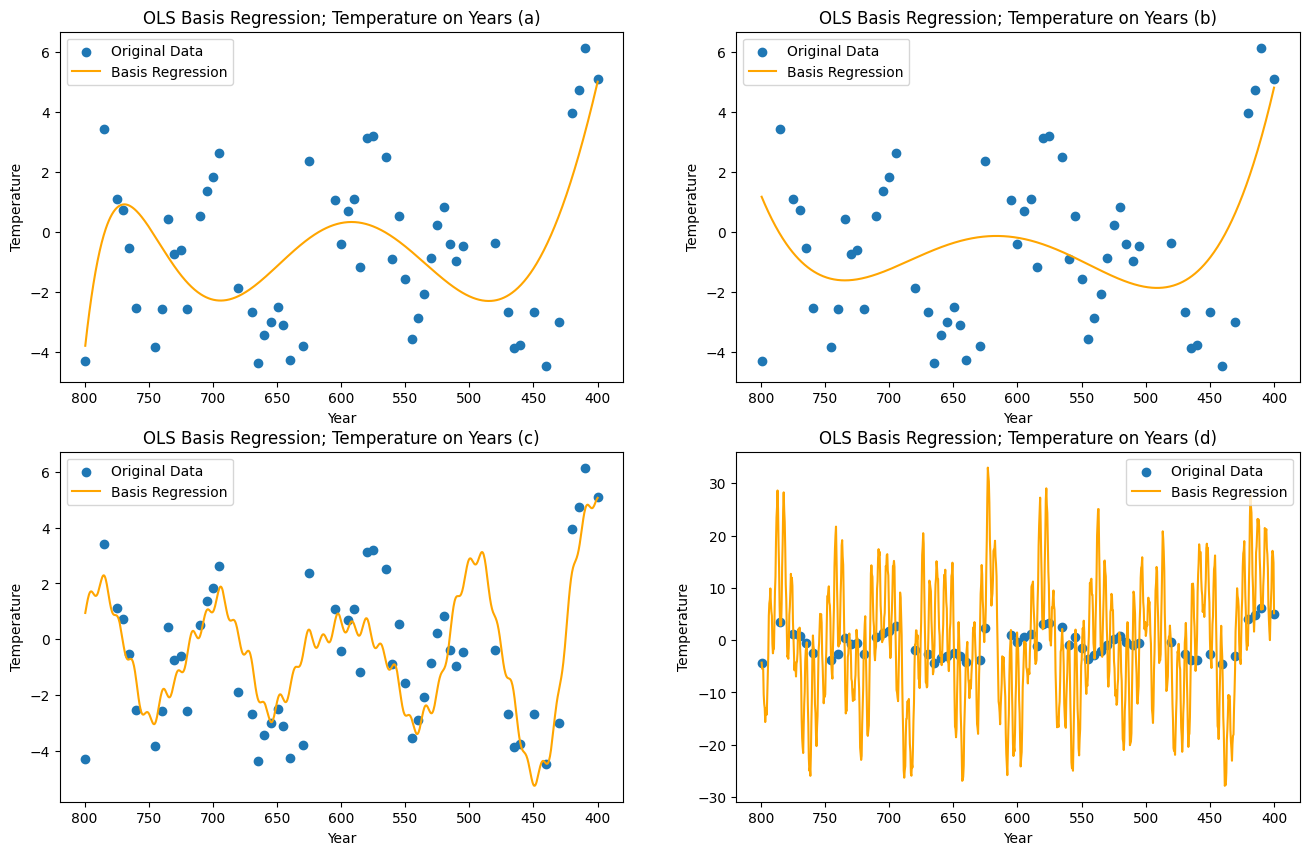
\includegraphics[scale=0.5]{hw1/linearRegressionGraph.png}\\
    \item
    \textbf{Part a:}\\
    Train MSE: 4.83; Test MSE: 7.96 \\
    Train Negative Log-Likelihood: 125.768; Test Negative Log-Likelihood: 63.256\\
    When looking at the graph this model seems to underfit our data because most of our data points are not covered (it is not accounting well to the noise in our data). Furthermore, our train MSE isn't that low meaning the data is not overfitting or optimally fitting our data points, and the MSE for our test data set is even worse. Additionally, our test negative log-likelihoods are high, indicating this model might not be optimal (interestingly, the train negative log-likelihood is higher than the test negative log-likelihood but this can be explained because our training data set is so much larger than our test data set).\\
    \\
    \textbf{Part b:}\\
    Train MSE: 5.53; Test MSE: 8.71 \\
    Train Negative Log-Likelihood: 129.620; Test Negative Log-Likelihood: 64.035 \\
    Again, when looking at the graph this model seems to underfit our data because most of our data points are not covered (it is not accounting well to the noise in our data). We see the same patterns as in part a with our train and test MSE's and our train and test negative log likelihoods (because they are both underfitting our data). \\
    \\
    \textbf{Part c:}\\
    Train MSE: 2.88; Test MSE: 5.97 \\
    Train Negative Log-Likelihood: 111.018; Test Negative Log-Likelihood: 62.098 \\
    Looking at the graph, this model seems to fit our data well. This is supported by the fact that our train MSE is really low and our test MSE and test log-likelihoods are the lowest of all of the different functions. Furthermore, the train and test MSE's do not diverge too much which indicates that we are not overfitting our data. \\
    \\
    \textbf{Part d:}\\
    Train MSE: 0.64; Test MSE: 58.90\\
    Train Negative Log-Likelihood: 68.303; Test Negative Log-Likelihood: 1162.188\\
    Looking at the graph, this model seems to overfit our data because it is hitting every single data point. This is backed up by our MSE values because our train MSE is very low (meaning we are really minimizing our error on the training data $\rightarrow$ overfitting) but our test MSE is really high meaning that this model does not fit our test data well. This model fits very specifically to the training data set.\\
    \\
    \item
    In this model we no longer need to share our entire training set with my friend because this model doesn't rely on the training data set (it is a parametric model). Instead we would just need to send them our weight vector and our basis function (how to transform a 1xD vector to a DxD vector) which means that the space complexity of storing this model would no longer depend on $N$ but instead it would depend on $D$. We would need to store our weight vector that's of dimension $D$ so our overall space complexity would be $O(D)$. Our time complexity is also going to depend on $D$. Our make$_$basis function takes $O(D)$ time because we need to transform the vector so we loop through it $D$ times and then we would need to multiply the transpose of our weight vector by this new vector which will take $O(D)$ time as well so our overall time complexity is $O(D)$.\\
    We can assume these complexities will be much smaller than those of the kNN and kernelized regressor because we would assume $N$ is much greater than $D$ (we would have significantly more data points than features of our data).\\ 

\end{enumerate}
%%%%%%%%%%%%%%%%%%%%%%%%%%%%%%%%%%%%%%%%%%%%%
% Problem 4
%%%%%%%%%%%%%%%%%%%%%%%%%%%%%%%%%%%%%%%%%%%%%
\newpage
\begin{problem}[Impact question: Building a descriptive (explanatory) linear regression model to understand the drivers of US energy consumption, to inform national policy decisions by the US President.]


\textbf{Prompt:} You are leading the machine learning team that is advising the US president. The US president is concerned about 3 things - climate change, the energy crisis in Europe and sustainable energy security in the US and asks you to help him understand what the driving factors of annual US energy consumption might be.  


How would you build a regression model that can be used to explain the driving factors of the annual US energy consumption? Please answer the questions below by using concise language (350 - 700 words). Bullet points are appropriate. 


This question is a conceptual question, and you are not required to implement the actual model. Yet, it is important that you think through your approach and its implications. 


\begin{enumerate}

\item \textbf{Target variable:} What target variable would you choose and what would be its unit? 
\item \textbf{Features:}  List 5 possible features and explain your assumption why you think they might impact the target variable. 
\item \textbf{Dataset size:} What should be the size of your dataset / covered time period? Why? 
\item \textbf{Performance metric:} What metric would you use to assess the model’s performance? 
\item \textbf{Policy decision:} Explain one policy decision the US president could make based on your model. 
\item \textbf{Trust:} What could be barriers for the US president to trust your model?  List two possible barriers. 
\item \textbf{Risk:} What happens if your model is wrong/inaccurate?  List one real-world consequence. 


\end{enumerate}

\end{problem}
\newpage
\textbf{Problem 4 Solution:}\\
\\
If I wanted to build a regression model that can be used to explain the driving factors of the annual US energy consumption I would choose to use US energy consumption as my target variable, and I would measure it in British Thermal Units. \\
\\
There are many possible features that we could use in this model, but I would focus on US population size, gas prices, average winter temperature, GDP per capita, and dollars spent on government subsidies for energy consumption in the previous year. Population size is an important metric because theoretically a larger population would consume more energy. As a result, if we were to see a spike in energy consumption, it would be important to know if it's because more people are consuming energy or another factor is impacting the change. Gas prices would also be helpful to look at because they could affect how much gas people use. If prices are higher, then people may try to limit their gas usage, driving down the total energy consumption. Additionally, average temperature in the winter is an important metric because colder temperatures would increase energy consumption for heating and other indoor activities. Furthermore, it would be interesting to look at how the US economy is doing (by examining GDP per capita) to understand how economic growth coincides with energy consumption. Lastly, it would be helpful to look at how the quantity of money the government spent on subsidized energy programs affects energy consumption to better see how the previous year's government policies were working. This could inform the President about whether they should continue the new program.\\
\\
I would choose my covered time period to be the last 50 years. I would like to cover enough years so that the model has a lot of data and we can better understand which features are affecting energy consumption the most. On the other hand, we don't want to go back too far in time because technology has changed so drastically and the world was so different (people had different priorities and it was much harder for different countries to communicate). If we go back too far, there could be many other factors affecting energy consumption and so our model may be more confusing. I believe 50 years is a good balance. This would mean my dataset would have a size of $50\cdot5 = 250$ because it would be the number of data points times the number of features.\\
\\
In order to assess the model's performance I would plan to use several tools. I would initially plan to try to minimize my MSE through cross validation and comparing different iterations of my model. Additionally, I would use bootstrapping in order to better understand the level of uncertainty in my model. \\
\\
The US president could use my model to possibly predict the US energy consumption for the next year. He could also use the model to determine if the previous year's subsidy programs were working. Using these results together, the president could decide to implement more energy consumption subsidies or taxation strategies.\\
\\
One barrier that could make it harder for the US president to trust my model is unpredictable events that happened in previous years that could impact the model. For example, COVID had a drastic effect on energy consumption, and it has had lasting effects so it could be risky to trust the model. Another barrier could be that the model is difficult to interpret and there are too many other factors that impact energy consumption. For example, foreign relations also play a big role in energy consumption as well as policy decisions about energy, so blindly trusting a model that is unable to adapt to those factors could be risky and lead to many other problems.\\
\\
If my model is wrong / inaccurate then it could possibly give a very inaccurate prediction of future energy consumption. This could drastically impact an expensive policy decision leading to more energy consumption. It could also affect the US relations with other countries creating other problems unrelated to energy consumption.


\newpage
%%%%%%%%%%%%%%%%%%%%%%%%%%%%%%%%%%%%%%%%%%%%%
% Name and Calibration
%%%%%%%%%%%%%%%%%%%%%%%%%%%%%%%%%%%%%%%%%%%%%
\subsection*{Name} Kara Siegel

\subsection*{Collaborators and Resources}
\textbf{Whom did you work with, and did you use any resources beyond cs181-textbook and your notes?}\\
Natalie Melas-Kyriazi, Noah Covey, Dominik Bohnet Zurcher

\subsection*{Calibration}
\textbf{Approximately how long did this homework take you to complete (in hours)? }\\
I spent approximately 15 hours on this problem set.

\end{document}
